% Figure 1 of the project summary: PlantIQ system architecture.
% Copied from IEEE-Paper/main.tex (figure fig:arch) so both documents show the same diagram.
% Build: ../IEEE-Paper/tools/tectonic.exe fig_arch.tex, then rasterise to 35_1.png (see make_figures.py).
\documentclass[border=6pt]{standalone}
\usepackage[T1]{fontenc}
\usepackage{newtxtext}
\usepackage{xcolor}
\usepackage{tikz}
\usetikzlibrary{arrows.meta,positioning,fit,backgrounds,calc,shapes.geometric}
\tikzset{
  box/.style={draw=black!70, rounded corners=2pt, align=center, font=\scriptsize, inner sep=3pt, fill=white},
  mod/.style={box, fill=blue!6, minimum width=2.45cm, minimum height=0.95cm},
  ext/.style={box, fill=black!4, dashed},
  arr/.style={-{Stealth[length=4pt]}, black!75, line width=0.5pt},
  grp/.style={draw=black!35, rounded corners=3pt, inner sep=5pt},
  grplabel/.style={font=\scriptsize\bfseries, black!70},
}
\begin{document}
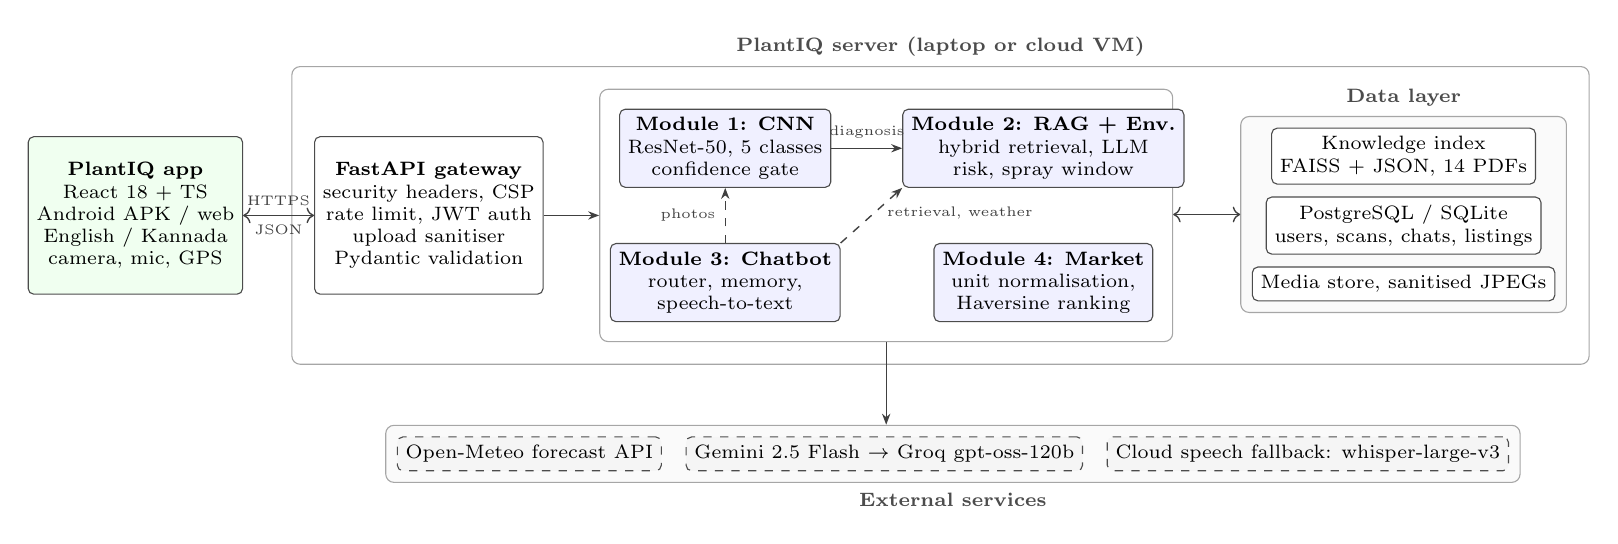
\begin{tikzpicture}
  % modules, 2 x 2 grid
  \node[mod] (m1) at (0,0) {\textbf{Module 1: CNN}\\ResNet-50, 5 classes\\confidence gate};
  \node[mod, right=9mm of m1] (m2) {\textbf{Module 2: RAG + Env.}\\hybrid retrieval, LLM\\risk, spray window};
  \node[mod, below=7mm of m1] (m3) {\textbf{Module 3: Chatbot}\\router, memory,\\speech-to-text};
  \node[mod, below=7mm of m2] (m4) {\textbf{Module 4: Market}\\unit normalisation,\\Haversine ranking};
  \draw[arr] (m1) -- node[above, font=\tiny]{diagnosis} (m2);
  \draw[arr, dashed] (m3) -- node[left, font=\tiny]{photos} (m1);
  \draw[arr, dashed] (m3.north east) -- node[pos=0.55, right, font=\tiny, xshift=1pt]{retrieval, weather} (m2.south west);
  % gateway and client
  \node[box, left=9mm of $(m1.west)!0.5!(m3.west)$, minimum width=2.2cm, minimum height=2.0cm] (gw)
       {\textbf{FastAPI gateway}\\security headers, CSP\\rate limit, JWT auth\\upload sanitiser\\Pydantic validation};
  \node[box, left=9mm of gw, minimum width=2.1cm, minimum height=2.0cm, fill=green!6] (app)
       {\textbf{PlantIQ app}\\React 18 + TS\\Android APK / web\\English / Kannada\\camera, mic, GPS};
  \draw[arr, <->] (app) -- node[above, font=\tiny]{HTTPS} node[below, font=\tiny]{JSON} (gw);
  % data layer (right of modules, inside the server)
  \node[box, minimum width=2.9cm, right=11mm of m2, yshift=-1mm] (kb) {Knowledge index\\FAISS + JSON, 14 PDFs};
  \node[box, minimum width=2.9cm, below=1.5mm of kb] (db) {PostgreSQL / SQLite\\users, scans, chats, listings};
  \node[box, minimum width=2.9cm, below=1.5mm of db] (fs) {Media store, sanitised JPEGs};
  % external services (row below the server)
  \coordinate (below) at ($(m3.south)!0.5!(m4.south)+(0,-1.45)$);
  \node[ext, anchor=north] (llm) at (below) {Gemini 2.5 Flash $\rightarrow$ Groq gpt-oss-120b};
  \node[ext, left=3mm of llm] (om) {Open-Meteo forecast API};
  \node[ext, right=3mm of llm] (stt) {Cloud speech fallback: whisper-large-v3};
  \begin{scope}[on background layer]
    \node[grp, fit=(m1)(m4), inner sep=7pt] (mods) {};
    \node[grp, fit=(kb)(fs), fill=black!2, inner sep=4pt] (data) {};
    \node[grp, fit=(om)(stt), fill=black!2, inner sep=4pt] (extg) {};
    \node[grp, fit=(gw)(mods)(data), inner sep=8pt, label={[grplabel]above:PlantIQ server (laptop or cloud VM)}] (srv) {};
  \end{scope}
  \node[grplabel, anchor=south] at (data.north) {Data layer};
  \node[grplabel, anchor=north] at (extg.south) {External services};
  \draw[arr] (gw.east) -- (gw.east -| mods.west);
  \draw[arr, <->] (mods.east |- data.west) -- (data.west);
  \draw[arr] (mods.south) -- (mods.south |- extg.north);
\end{tikzpicture}
\end{document}
